\section{Análise descritiva dos lobistas}
\label{sec:resultados_descritica_lobistas}
A Tabela \ref{tab:dist_orgs_reunioes} apresenta a distribuição de lobistas e sua atividade (mensurada pelo número de reuniões) por categoria organizacional. Os dados revelam uma predominância de interesses empresariais, que constituem o maior grupo tanto em número de organizações (2.409) quanto em volume de reuniões (22.427). Em média, cada organização empresarial realizou 9,31 reuniões, a maior taxa entre as categorias. As ONGs figuram como o segundo grupo mais ativo, seguidas pela categoria "Outros".

\begin{table}[!htbp]
\centering
\caption{Distribuição de organizações, reuniões e reuniões por lobista, por categoria de organização}
\label{tab:dist_orgs_reunioes}
\begin{tabular}{lccc}
\hline
Categoria & Organizações & Reuniões & Reuniões por Organização \\
\hline
Empresarial & 2.409 & 22.427 & 9,31 \\
ONGs & 1.271 & 10.966 & 8,63 \\
Outros & 1.042 & 6.950 & 6,67 \\
\hline
Total & 4.722 & 40.343 & 8,54 \\
\hline  
\end{tabular}
\end{table}

Esses resultados corroboram uma vasta literatura que aponta para a assimetria de recursos e representação no universo do lobby. Interesses empresariais, que dispõem de maiores recursos financeiros, tendem a predominar na atividade de lobby \cite{de_figueiredo_advancing_2014}. No contexto específico da União Europeia, estudos demonstram que grupos empresariais e associações nacionais são os mais presentes \cite{dur20212wholobbies, eising2007institutional}, o que levou alguns autores a caracterizarem o sistema como um "pluralismo de elite" \cite{coen1997evolution, schmidt2006procedural}.

A intensidade da atividade, refletida no elevado número total de reuniões (40.343), sinaliza uma forte competição pelo acesso aos tomadores de decisão, um recurso considerado escasso pela literatura \cite{hall1990buying}. Embora os atores empresariais detenham a dianteira, a presença expressiva de ONGs indica um ambiente competitivo, e não monolítico. Essa coexistência sugere que diferentes tipos de organizações mobilizam recursos distintos para influenciar o processo político. Enquanto interesses empresariais podem alavancar recursos financeiros e expertise técnica, ONGs e outros grupos da sociedade civil podem recorrer a recursos como legitimidade, representatividade e apoio público para defender suas causas \cite{Coen2019, dur_measuring_2008}.

Portanto, a análise descritiva inicial já delineia uma das tensões centrais investigadas neste trabalho: o desequilíbrio de poder e recursos entre interesses empresariais e outros setores da sociedade, e como essa assimetria se manifesta na competição por influência política no Parlamento Europeu.


% Análise do orçamento máximo declarado
A análise do orçamento máximo declarado por categoria (Figura \ref{fig:budget_ln_boxplot}), em escala logarítmica, revela padrões distributivos distintos. O grupo empresarial, embora mais numeroso em quantidade de organizações, exibe a menor mediana de orçamento e uma distribuição notavelmente mais concentrada, o que sugere uma maior homogeneidade nos gastos com lobby declarados por essas entidades.

Em contrapartida, as ONGs e a categoria "Outros" apresentam medianas mais elevadas e uma variância substancialmente maior. Essa dispersão indica uma forte heterogeneidade interna, sugerindo a coexistência de organizações com recursos modestos e outras com orçamentos muito elevados, que influenciam a distribuição.

\begin{figure}[!htbp]
\centering
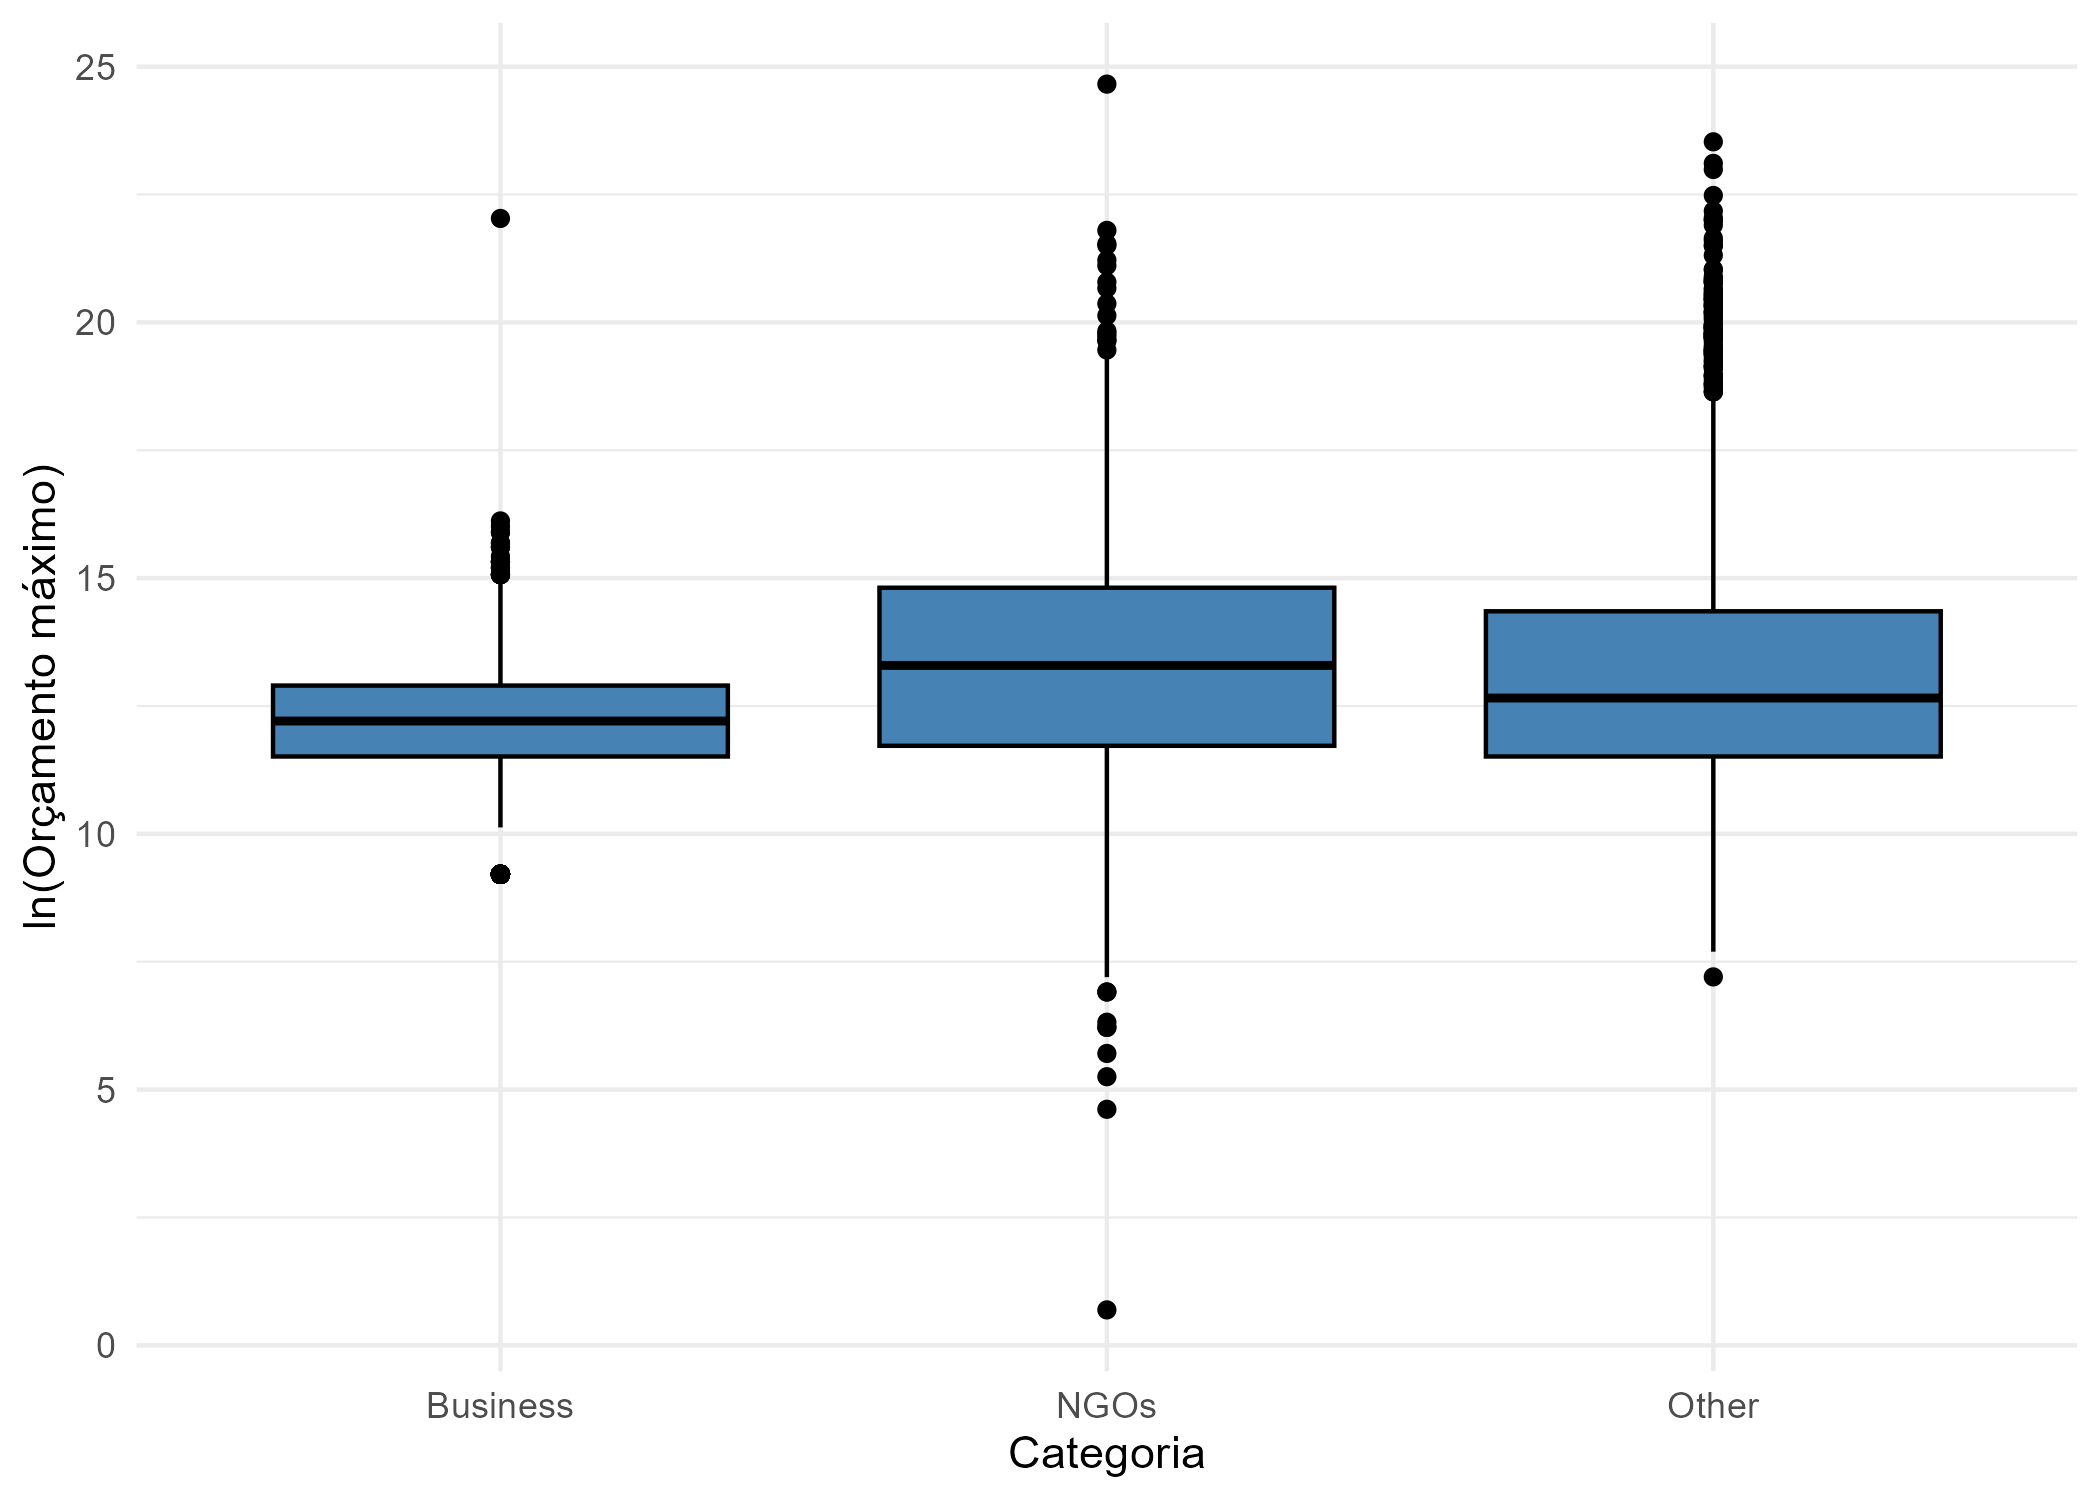
\includegraphics[width=0.75\textwidth]{figures/descriptives_lobbyists/boxplot_max_budget_by_category.png}
\caption{Distribuição de orçamento máximo declarado ($ln(Orçamento Maximo Declarado)$) por categoria}
\label{fig:budget_ln_boxplot}
\end{figure}

Este achado é particularmente interessante, pois parece tensionar a premissa da literatura de que interesses empresariais dominam em termos de recursos financeiros \cite{de_figueiredo_advancing_2014, dur20212wholobbies}. Uma interpretação possível é que a categoria empresarial seja composta por um grande número de atores com gastos mais padronizados, enquanto as categorias de ONGs e "Outros" contêm algumas organizações "gigantes", cujos orçamentos massivos podem refletir campanhas de alto custo ou estruturas de financiamento distintas. A alta variância pode, ainda, ser um reflexo de diferentes estratégias: enquanto empresas podem ter um dispêndio mais constante, ONGs podem mobilizar grandes somas para temas de alta saliência, onde a opinião pública é um fator crucial \cite{mahoney_lobbying_2007}.

Adicionalmente, a concentração no grupo empresarial pode estar relacionada ao problema da ação coletiva \cite{olson1971logic}, onde muitas empresas optam por atuar por meio de associações — que podem estar classificadas na categoria "Outros". De todo modo, os dados reforçam que a relação entre recursos financeiros e influência não é direta \cite{simon_notes_1953}, e que a capacidade de mobilizar diferentes tipos de recursos — não apenas financeiros, mas também de legitimidade e informação \cite{Coen2019} — é central para a dinâmica do lobby na UE.


% Distribuição geográfica
A análise da distribuição geográfica dos lobistas (Figura \ref{fig:country_distribution}) revela uma acentuada concentração em polos institucionais da União Europeia, com Bélgica (24,2\%), Alemanha (15,3\%) e França (10,1\%) abrigando a maioria das organizações. Este padrão corrobora a tese da vantagem da proximidade institucional: a presença massiva na Bélgica, sede da Comissão Europeia e de grande parte das atividades do Parlamento, e na França, que sedia as sessões plenárias do Parlamento em Estrasburgo, é uma resposta estratégica à complexa governança multinível da UE \cite{richardson2000government}.

\begin{figure}[!htbp]
\centering
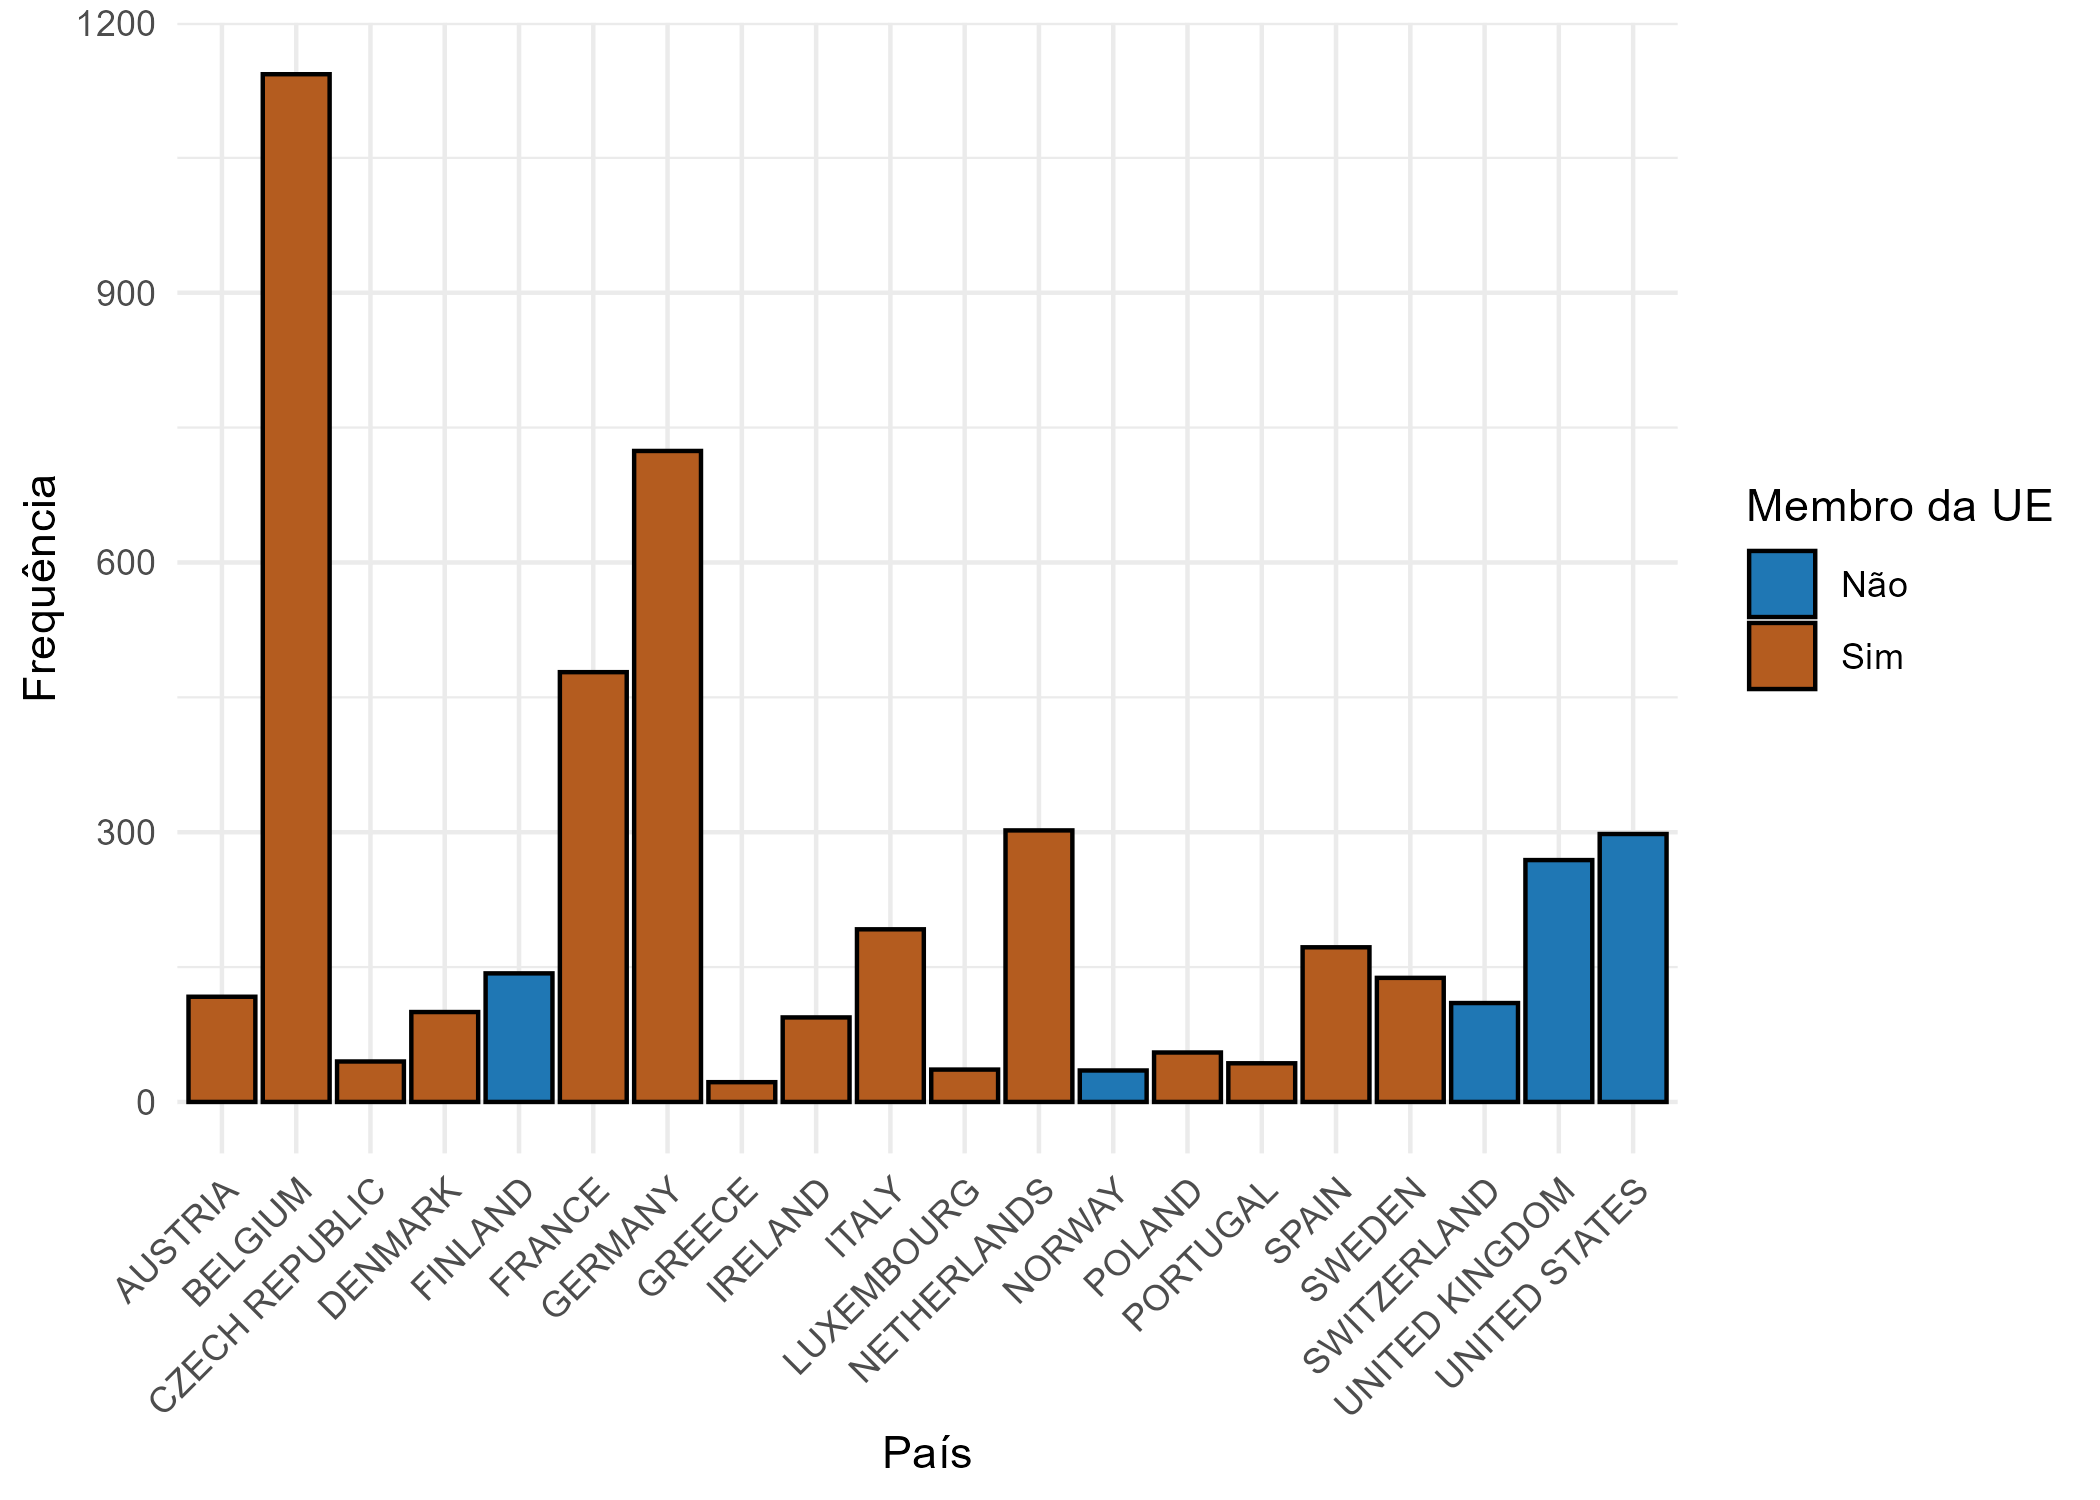
\includegraphics[width=0.9\textwidth]{figures/descriptives_lobbyists/barplot_country_distribution.png}
\caption{Top 20 países-sede (n = 4.516 organizações, totalizando 95,6\% do total de organizações)}
\label{fig:country_distribution}
\end{figure}

O fenômeno do \textit{venue-shopping} — a escolha estratégica do fórum mais favorável para exercer pressão — é central para entender essa distribuição \cite{kluver2015legislative}. A estrutura institucional da UE, com poder decisório partilhado entre a Comissão, o Conselho e o Parlamento, incentiva os grupos de interesse a se estabelecerem nos locais onde podem monitorar e intervir mais eficazmente no ciclo político. A proeminência de países como Alemanha e França reflete não apenas a proximidade, mas também o peso político e econômico que exercem dentro da União.

Adicionalmente, a presença significativa de atores extracomunitários, que representam cerca de 20\% do total de organizações com sedes em 70 países (com destaque para os Estados Unidos, com 6,3\%), evidencia a importância da UE como arena regulatória global. A atratividade do mercado europeu e o impacto de suas decisões incentivam atores internacionais a investir em uma presença local para influenciar a formulação de políticas que afetarão seus interesses. O recorte do top 20, que mostra uma cauda longa com muitos países de baixa frequência, reforça a ideia de que, embora o sistema seja permeável, os altos custos de manter uma operação de lobby eficaz na Europa centralizam a influência em atores com maiores recursos e localização estratégica.

% Distribuição temporal dos registros
Temporalmente, observa-se aceleração do registro de entidades após meados da década de 2010, com 2023 concentrando 17,9\% do total. Picos intermediários (2015--2016; 2020--2022) são compatíveis com ciclos legislativos, janelas regulatórias e alterações incrementais nos mecanismos de transparência.

\begin{figure}[!htbp]
\centering
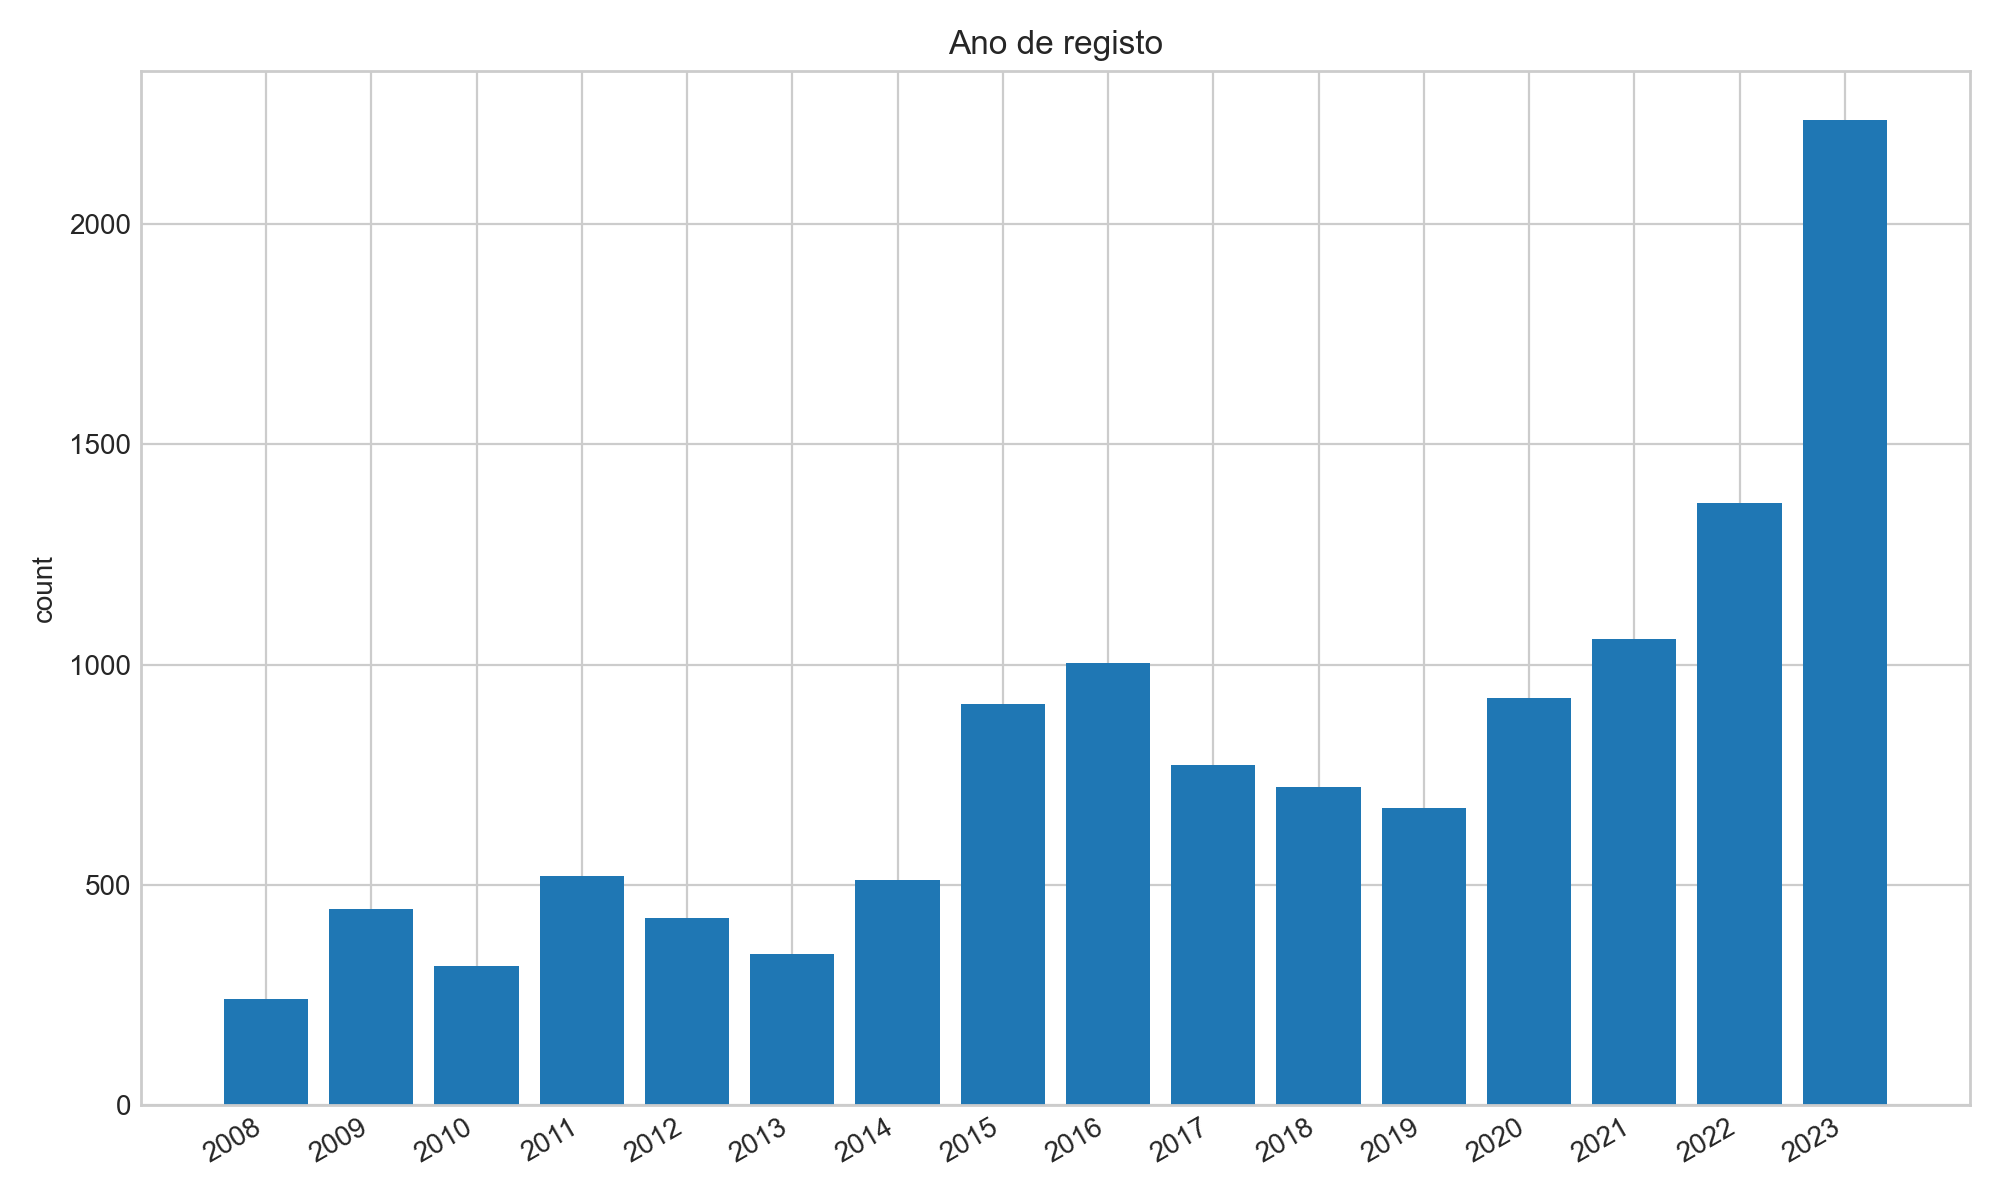
\includegraphics[width=0.75\textwidth]{figures/year_distribution.png}
\caption{Ano de registo}
\end{figure}

O padrão visual sugere crescimento estrutural recente do ecossistema de representação de interesses, possivelmente associado às agendas de transição digital e verde e à recomposição pós-pandemia.

% Distribuição temática
As incidências por domínio (Figura \ref{fig:theme_coverage}) destacam \textit{Infraestrutura e Indústria} (68,3\%), \textit{Tecnologia} (67,9\%) e \textit{Economia e Comércio} (67,4\%), seguidas por \textit{Ambiente e Clima} (64,7\%) e \textit{Assuntos Externos e Segurança} (51,3\%). Temas como \textit{Saúde} (43,7\%) e \textit{Educação} (41,2\%) são intermediários; \textit{Agricultura} (35,3\%) e \textit{Direitos Humanos} (25,3\%) têm menor incidência relativa.

\begin{figure}[!htbp]
\centering
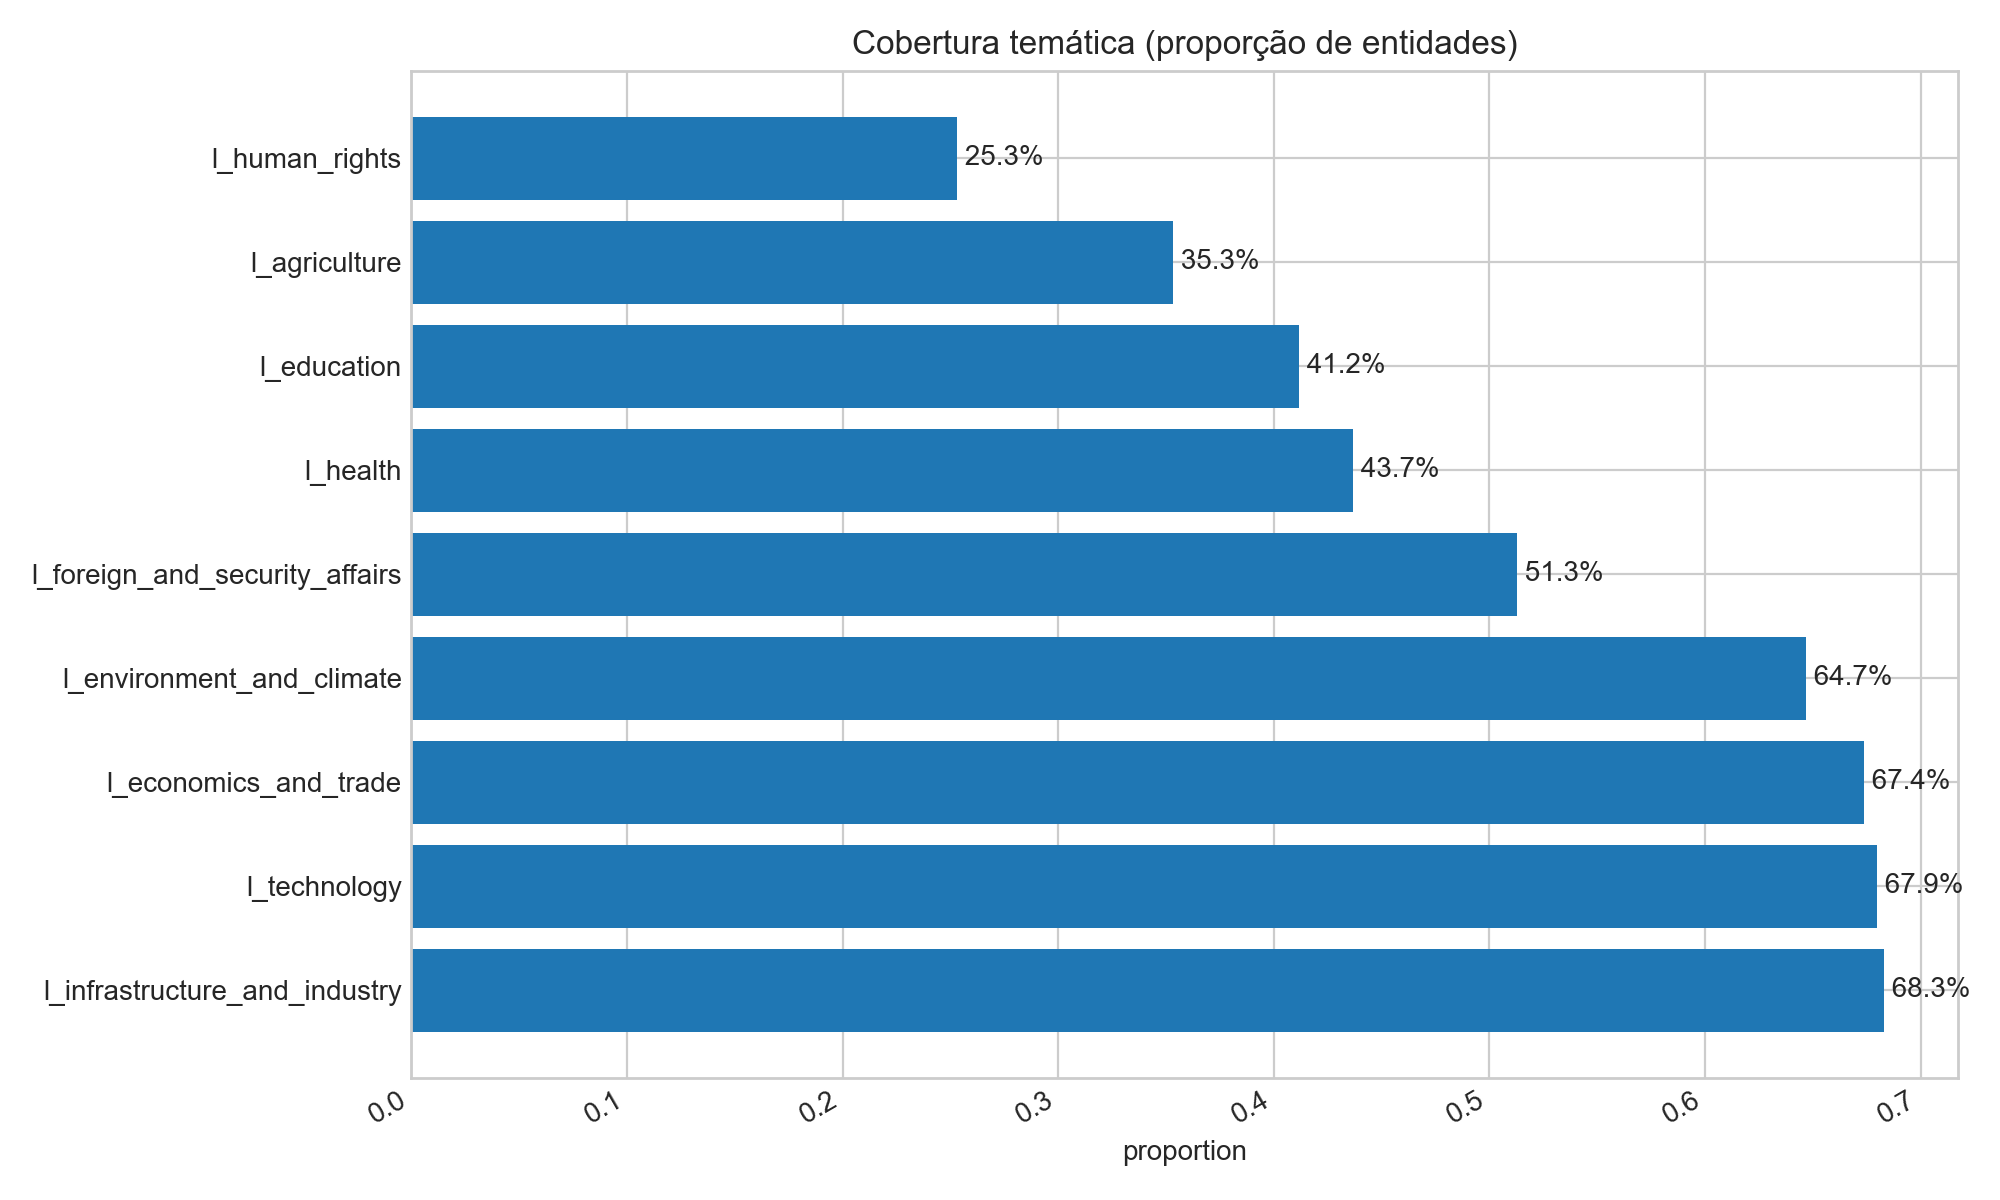
\includegraphics[width=0.9\textwidth]{figures/theme_coverage.png}
\caption{Cobertura temática (proporção de entidades)}
\label{fig:theme_coverage}
\end{figure}

O ordenamento por proporção sugere centralidade de agendas de competitividade industrial, digitalização e cadeias de valor, bem como a transversalidade da pauta ambiental.


\begin{figure}[!htbp]
\centering
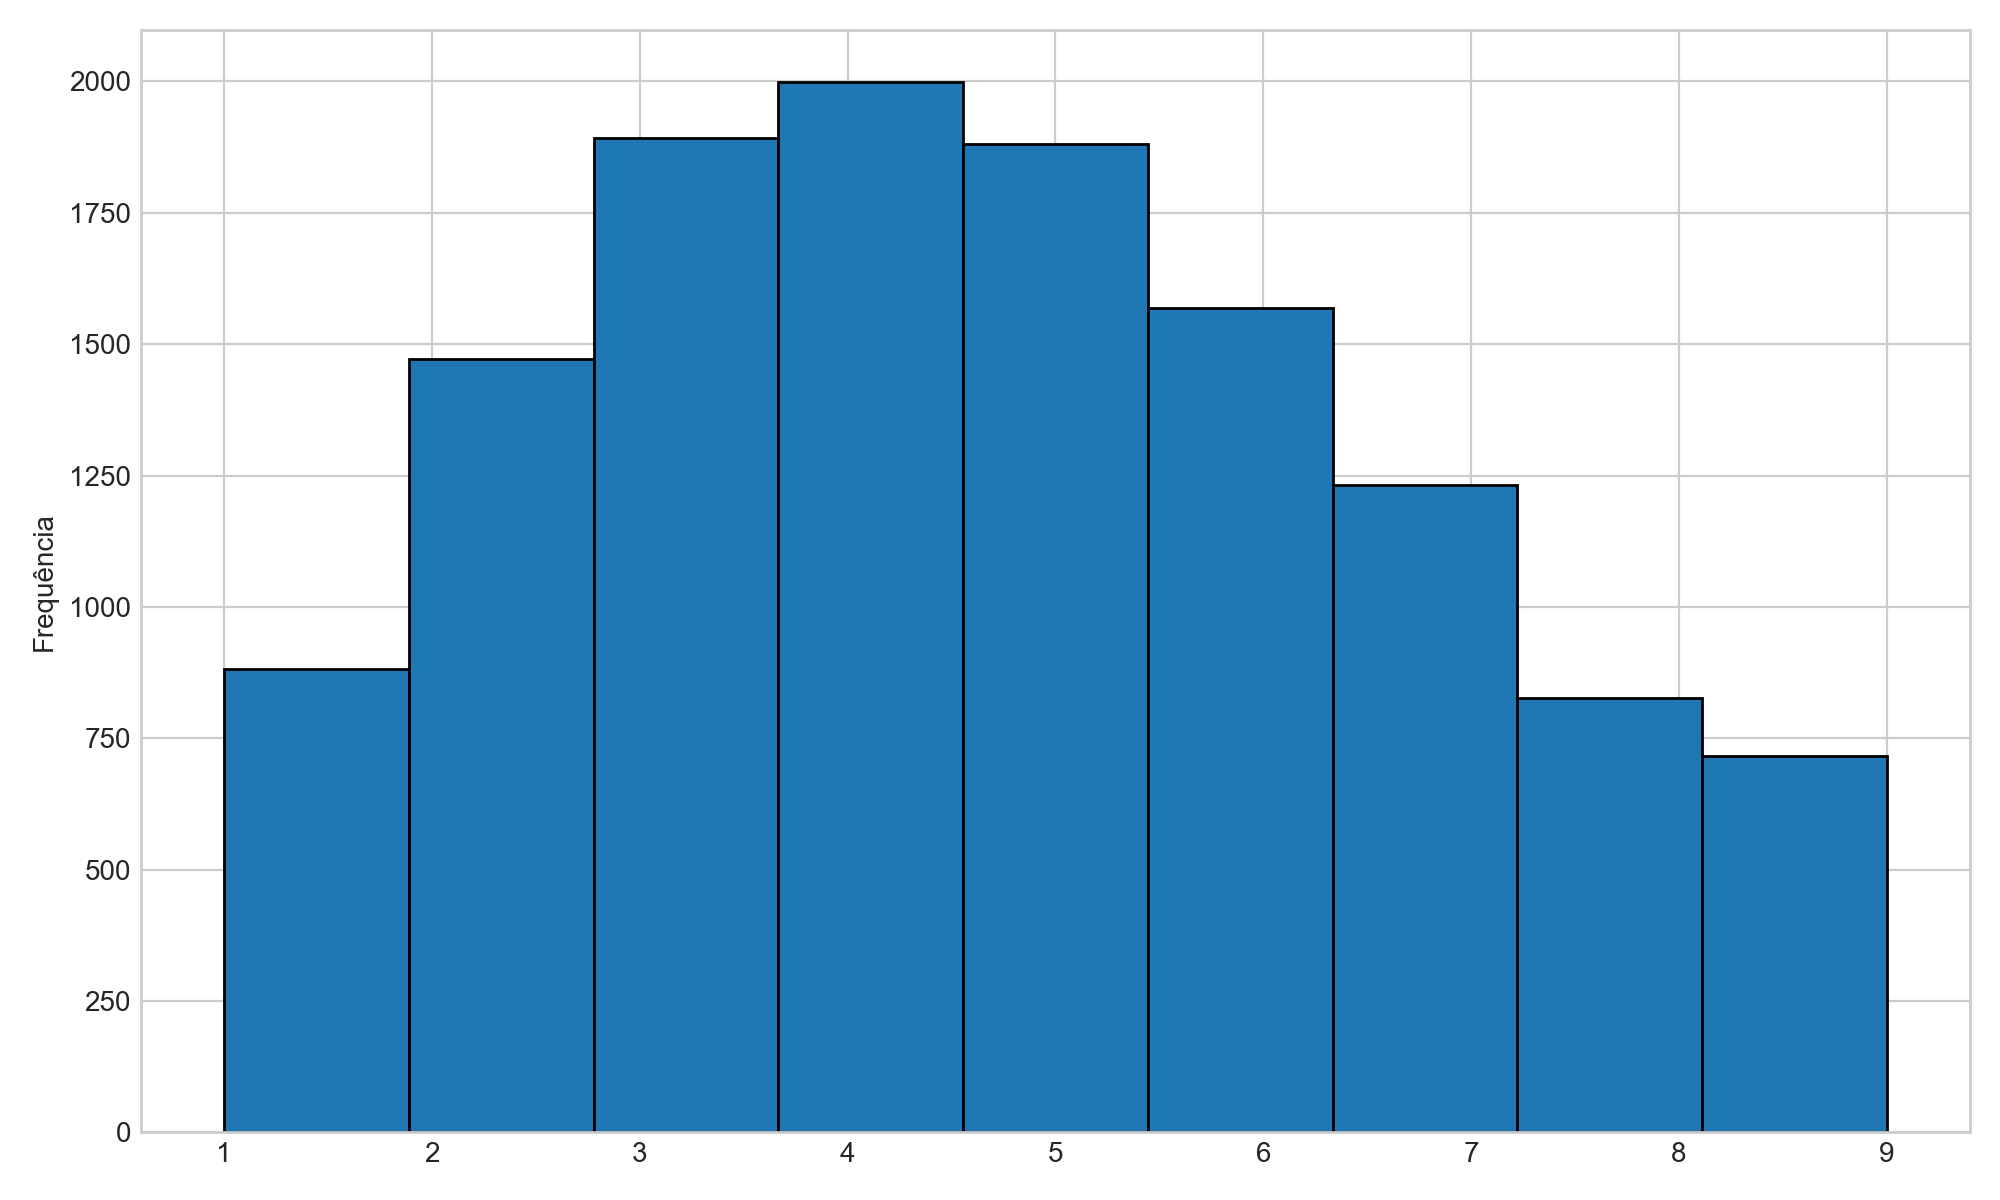
\includegraphics[width=0.75\textwidth]{figures/themes_per_lobbyist_hist.png}
\caption{Número de temas por lobista}
\label{fig:themes_per_lobbyist_hist}
\end{figure}

A distribuição do número de temas por entidade (Figura \ref{fig:themes_per_lobbyist_hist}) indica a coexistência de atores multi-temáticos e especializados. Esse traço é relevante para a modelagem, pois sugere que a intensidade de esforço (extensivo vs. intensivo) varia com o perfil organizacional e o ambiente regulatório dos domínios.




Em conjunto, os resultados descritivos apontam para um ecossistema plural, geograficamente ancorado em polos institucionais centrais, com dinamismo temporal recente e agendas orientadas por digitalização, competitividade industrial e sustentabilidade. Esses padrões informam as escolhas de especificação nos capítulos seguintes, notadamente a estratificação por perfis organizacionais, a construção de domínios temáticos e o controle para tendências temporais.


Os resultados descritivos delineiam um panorama abrangente do universo de lobistas registados junto às instituições europeias. Em primeiro lugar, a distribuição por categoria revela a coexistência de diferentes perfis organizacionais (\textit{Business}, \textit{NGOs} e \textit{Other}), com magnitudes comparáveis entre atores empresariais e organizações da sociedade civil. Essa composição é compatível com a literatura sobre pluralismo organizacional e competição por acesso institucional no contexto da União Europeia, sugerindo um campo de ação onde interesses difusos e concentrados buscam simultaneamente agenda e influência.

No plano geográfico, observa-se forte concentração em Estados-Membros centrais e com infraestrutura institucional robusta. Destacam-se Bélgica (18,2\%), Alemanha (14,0\%) e França (9,3\%), seguidas por Países Baixos, Espanha, Reino Unido e Itália (6\% cada). Há ainda presença extracomunitária não desprezível (Estados Unidos 4,5\%), o que evidencia a atratividade regulatória do mercado europeu e a permeabilidade do \textit{lobbying} transnacional. Esses achados são consistentes com hipóteses de \textit{venue shopping} e vantagens de proximidade institucional (Bruxelas/Strasburgo) para atividades de representação de interesses.

Temporalmente, as frequências por ano indicam aceleração recente dos registos, com 2023 concentrando 17,9\% das entradas no período observado. Picos intermediários (2015--2016; 2020--2022) são compatíveis com ciclos legislativos, janelas regulatórias e mudanças incrementais no regime de transparência, fatores que tendem a alterar a propensão ao registro. A expansão no pós-2020 pode refletir a reconfiguração de estratégias após as restrições pandémicas, além da ênfase em agendas de transição digital e verde.

Quanto à cobertura temática, a incidência é mais elevada em \textit{Infraestrutura e Indústria} (68,3\%), \textit{Tecnologia} (67,9\%) e \textit{Economia e Comércio} (67,4\%), seguidas por \textit{Ambiente e Clima} (64,7\%) e \textit{Política Externa e Segurança} (51,3\%). Temas como \textit{Saúde} (43,7\%) e \textit{Educação} (41,2\%) ocupam posição intermediária, ao passo que \textit{Agricultura} (35,3\%) e \textit{Direitos Humanos} (25,3\%) apresentam menor incidência relativa. Em conjunto, esse perfil sugere: (i) centralidade de agendas de competitividade industrial, digitalização e cadeias de valor; (ii) transversalidade da pauta ambiental como condicionante regulatória; e (iii) segmentação de atores com missões setoriais mais estreitas ou normativas, potencialmente menos numerosos.

A distribuição do número de temas por lobista sugere coexistência de atores multi-temáticos, capazes de cobrir diversas frentes de política pública, e de atores especializados com foco estreito. Tal heterogeneidade é relevante para a modelagem empírica, pois a intensidade de esforço (extensivo vs. intensivo) pode variar sistematicamente com o tipo de organização e com o ambiente regulatório dos diferentes domínios.

No que se refere ao orçamento máximo declarado (em log natural), as medidas-resumo apontam mediana próxima de 11,5 e quartis aproximados entre 10,1 e 12,9. Identificam-se valores inválidos/extremos na base administrativa (por exemplo, ocorrências infinitas), que distorcem a média e o desvio-padrão; por isso, a interpretação deve privilegiar estatísticas robustas (mediana e intervalos interquartílicos) e, quando pertinente, rotinas de limpeza e estratégias robustas nos exercícios inferenciais. Substantivamente, a dispersão é compatível com a coexistência de grandes associações/empresas e organizações de menor porte, com implicações para capacidades de acesso e agenda-setting.

Em síntese, as evidências descritivas apontam para um ecossistema plural, geograficamente ancorado em polos institucionais centrais, com dinamismo temporal recente e agendas orientadas por digitalização, competitividade industrial e sustentabilidade. Esses padrões informam as escolhas de especificação nos capítulos seguintes, notadamente a estratificação por perfis organizacionais, a construção de domínios temáticos e o controle para tendências temporais.

